\chapter{Power radiated by the Hertz dipole}
In the approach to find the power radiated, we would first find out the poynting vector for the dipole and the power can be gotten by integrating the poynting vector 
over the total surface enclosing the antenna. 

The average poynting vector $\bar{P}_{av} = \dfrac{1}{2}\mathfrak{Re}\{\bar{E} \times \bar{H}^*\} $\\

Here, we are considering the total fields produced by the dipole
$$
= \dfrac{1}{2}\mathfrak{Re}\{E_\theta H_\phi\hat{\theta} \times \hat{\phi} + E_r H_\phi\hat{r}\times \hat{\theta}\}
$$
$$\fbox{$
= \dfrac{1}{2}\mathfrak{Re}\{E_\theta H_\phi^*\hat{r} - E_r H_\phi^*\hat{\theta}$\} }\footnote{\label{cross product note}since \ $\hat{\theta}\times\hat{\phi} = \hat{r} \ and \ \hat{r}\times\hat{\phi} = -\hat{\theta}$}
$$
From equation *,* and *
\begin{align*}
E_r &= \dfrac{I_\circ d\ell\cos\theta e^{j(\omega t - \beta r)}}{2\pi\omega\epsilon}\left(\dfrac{\beta}{r^2} - \dfrac{j}{r^3}\right)\\  
E_\theta &= \dfrac{I_\circ d\ell\sin\theta e^{j(\omega t - \beta r)}}{4\pi\epsilon}\left(\dfrac{j\beta^2}{\omega r} + \dfrac{\beta}{\omega r^2} - \dfrac{j}{\omega r^3}\right)\\    
 H_\phi^* &= \dfrac{I_\circ d\ell\sin\theta e^{j(\omega t - \beta r)}}{4\pi}\left(\dfrac{1}{r^2} - \dfrac{j\beta}{r}\right)
\end{align*}
\paragraph{}
The $E_rH_\phi^*$ gives a purely imaginary term as follows
$$\left(\dfrac{\beta}{r^2} - \dfrac{j}{r^3}\right)\left(\dfrac{1}{r^2} 
 - \dfrac{j\beta}{r}\right)$$
$$=  \dfrac{\beta}{r^4} - \dfrac{j\beta^2}{r^3} 
- \dfrac{j}{r^5} - \dfrac{\beta}{r^4} $$
$$= -j\left( \dfrac{\beta}{r^3}  +  \dfrac{1}{r^5}\right) $$
so we completely neglect it. Now let us consider the $E_\theta H_\phi^*$ term;
$$\left(\dfrac{j\beta^2}{\omega r} + \dfrac{\beta}{\omega r^2} - \dfrac{j}{\omega r^3}\right)\left(\dfrac{1}{r^2} - \dfrac{j\beta}{r}\right)$$
$$\Longrightarrow \dfrac{j\beta^2}{\omega r^3} 
+ \dfrac{\beta^3}{\omega r^2} + \dfrac{\beta}{\omega r^4} 
- \dfrac{j\beta^2}{\omega r^3} - \dfrac{j}{\omega r^5}
- \dfrac{\beta}{\omega r^4}$$
$$\Longrightarrow \dfrac{\beta^3}{\omega r^2} - \dfrac{j}{\omega r^5}$$
Thus \quad  
\begin{dmath*}
\bar{P}_{av} = \dfrac{1}{2}\mathfrak{Re}\left[\left(\dfrac{I_\circ d\ell\sin\theta}{4\pi}\right)^2\dfrac{1}{\epsilon} \left(\dfrac{\beta^3}{\omega r^2} - \dfrac{j}{\omega r^5}\right)\hat{r}\right]
= \dfrac{1}{2}
\left[\dfrac{I_\circ d\ell\sin\theta}{4\pi r}\right]^2 \dfrac{\beta^3}{\epsilon\omega}\hat{r} 
\end{dmath*}
Notice that the terms that contributed to the power density were the radiation fields, the other terms only contributed to the reactive component of power. From the calculation, we observed that the $\theta$  component of the poynting vector was purely imaginary which means that power oscillates one half cycle in the positive $\theta$ direction and the other half cycle in the negative $\theta$ direction. So the power keeps oscillating but there is no net power flow in the $\theta$ diretion.

Since one problem with the Hertz dipole is a symmetrical problem, the Hertz dipole is not having any preferred direction of current flow and so there would not be any preferred direction for the power to flow. Hence, the power essentially will flow radially outwards.

Now, to determine the total power we would integrate the poynting vector over a closed surface enclosing the Hertz dipole.
\begin{figure}[h]
\centering
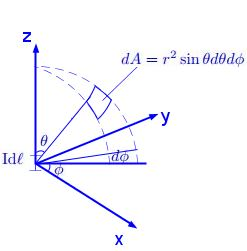
\includegraphics[width=.8\linewidth]{./graphics/diagram1}
\caption{Elemental area in spherical coordinate}
\label{figure12}
\end{figure}

Total power $ W = \int^{2\pi}_0 \int^\pi_0 P_{av}r^2\sin\theta d\theta d\phi $
$$
= \int^{2\pi}_0\int^\pi_0 \dfrac{1}{2}
\left[\dfrac{I_\circ d\ell\sin\theta}{4\pi}\right]^2\dfrac{\beta^3}{\epsilon\omega}\sin\theta d\theta d\phi
$$
Notice that $r^2$ cancels out showing the total power radiated by the dipole is not a function of what size of sphere is used
\begin{align*}
&= \dfrac{1}{2}\int^\pi_0 (2\pi) 
\left[\dfrac{I_\circ d\ell\sin\theta}{4\pi}\right]^2
\dfrac{\beta^3}{\epsilon\omega}\sin\theta d\theta\\\\
&= \left[\dfrac{I_\circ d\ell}{4\pi}\right]^2\dfrac{\beta^3\pi}{\epsilon\omega}
\int^\pi_0\sin^3\theta d\theta\\\\
W &= \left(\dfrac{I_\circ d\ell}{4\pi}\right)^2\dfrac{\beta^3\pi}{\omega\epsilon}
\int^\pi_0\sin^2\theta\sin\theta d\theta\\\\
&= \left(\dfrac{I_\circ d\ell}{4\pi}\right)^2\dfrac{\beta^3\pi}{\omega\epsilon}
\int^\pi_0\left(1 - \cos^2\theta\right)\sin\theta d\theta 
\end{align*}
Let $ \cos\theta  = t \Longrightarrow -\sin\theta d\theta = dt$
\begin{align*}
W&= \left(\dfrac{I_\circ d\ell}{4\pi}\right)^2\dfrac{\beta^3\pi}{\omega\epsilon}
\int^{-1}_1(1 - t^2)(-dt)\\\\
&= \left(\dfrac{I_\circ d\ell}{4\pi}\right)^2\frac{\beta^3\pi}{\omega\epsilon}
\int^1_{-1}(1 - t^2)dt\\\\
&= \left(\dfrac{I_\circ d\ell}{4\pi}\right)^2\dfrac{\beta^3\pi}{\omega\epsilon}
\left(t - \dfrac{t^3}{3}\bigg\vert^1_{-1}\right)\\\\
&= \left(\dfrac{I_\circ d\ell}{4\pi}\right)^2\dfrac{\beta^3\pi}{\omega\epsilon} \times \dfrac{4}{3}\\\\
&= \dfrac{I_\circ^2(d\ell)^2\beta^3\pi}{16\pi^2\omega\epsilon} \times \dfrac{4}{3}\\\\
&= \dfrac{I_\circ^2(d\ell)^2\beta^3}{12\pi\omega\epsilon}
\end{align*}
Recall, $\beta = \omega\sqrt{\mu\epsilon}$ and $\beta = \dfrac{2\pi}{\lambda}$
$$\dfrac{\beta}{\omega\epsilon} = 
\dfrac{\beta \times \beta^2}{\omega\epsilon}
 = \dfrac{\omega\sqrt{\mu\epsilon}}{\omega\epsilon}
 \left(\dfrac{2\pi}{\lambda}\right)^2
  = \dfrac{4\pi^2}{\lambda^2}\eta$$
 substituting back into the expression for W gives:
\begin{align}
\fbox{$ W = 40\pi^2I_\circ^2\left(\dfrac{d\ell}{\lambda}\right)^2$} \footnote{ \label{note for intrinsic impedance of free space} $where \ \eta = 120\pi \ for \ free \ space$}
\end{align}
Recall $I_\circ$ is the peak current and in the expression, the power is proportional to the square of the current. Also, We note that the power radiated is related to the square of the length of the dipole normalized to the value of the wavelength$(\lambda)$, which means the absolute length of the dipole is not important but what is important is the relative length of the dipole with respect to the wavelength. So increasing the lenght d$\ell$ should increase the power generated, well, this is not completely true because there is a range to which the length of the hertz dipole can be increased. For the assumption of uniform current distribution in the Hertz dipole, the length should be far less than the wavelength of the time varying signal ($d\ell \ll \lambda$). Thus, as long as the uniformity of current is maintained and the current element can be called a Hertz dipole, then increasing the length will increase the power generated. 
 
 Due to the dual nature of the antenna, let us observe what happens from the circuit point of view when power is radiated. Let us assume that the Hertz dipole is connected to a voltage source as shown in figure \ref{figure13}.
\begin{figure}[h]
\centering
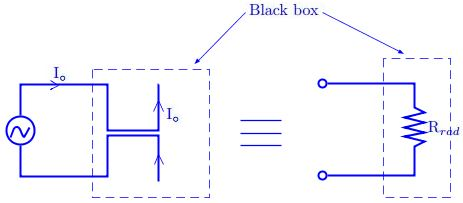
\includegraphics[width=1\linewidth]{./graphics/diagram2}
\caption{Radiation resistance model}
\label{figure13}
\end{figure}

The voltage source supplies current $I_\circ$ to the dipole and the dipole radiates power away from its structure. If the dipole is enclosed in a black box and the characteristics are observed through the terminals, the box will consume power and so the black box will appear as a resistance which is the characteristic. The power consumed by the black box would be equal to the power radiated by the dipole. We denote this resistance by $R_{rad}$ called radiation resistance. Note that the black box acts as a resistor because we are considering only the radiation fields which contribute to the power flow. So, $\dfrac{1}{2}I_\circ^2R_{rad} = W = 40\pi^2I_\circ^2\left(\dfrac{d\ell}{\lambda}\right)^2$ 
\begin{align}
\fbox{ $ R_{rad} = 80\pi^2\left(\dfrac{d\ell}{\lambda}\right)^2$}
\end{align}

If we consider all fields produced by the Hertz dipole, then the black box will be modeled by an impedance $Z = (R + jX)\Omega$. 

From the expression in equation 1.1 above, it is seen that the power radiated is proportional to $R_{rad}$ for a given current, hence the higher the radiation resistance, the more the power radiated by the Hertz dipole. Also, from the expression, it suggests that the larger the length of the dipole, the larger the resistance but $d\ell$ can only be increased to a limited range. For instance, let the length of the dipole be about 10\%\ of the wavelength ($d\ell = 0.1\lambda$) to satisfy the condition of $d\ell \ll \lambda$. Substituting the value $d\ell = 0.1\lambda$ in the equation 1.1, we have that $R_{rad}$ is approximately $8\Omega$ ($R_{rad} \cong 8\Omega$) which is a very small resistance and thus the efficiency of the antenna is likely to be too low. Effective matching to the source (dipole) also becomes very difficult to achieve as practical transmission lines have characteristic impedance in the range of ten - a few hundred ohms. 
 \paragraph{}
 In conclusion, radiation resistance is a good concept when estimating the power radiated by a given antenna and then by devising the mechanism by which the radiation resistance can be increased, we can radiate more power for a given current in the antenna. 
 
 \section{Radiation Patterns}
 In this section, we will observe the directional characteristics of the Hertz dipole. In analysing the directional characteristics of an antenna, we concern ourselves with the variation of fields with respect to the $\theta \ and \ \phi$ angles in the spherical coordinate system. In order to get the directional characteristics, we need a plot of the fields in 3D surface as a function of $\theta \ and \ \phi$ which is called the radiation pattern of the antenna. 
 
 \paragraph{}
 To simplify our analysis when considering these components $E_\theta \ and \ H_\phi$, as we are concerned with only the radiation fields, we will treat the $I_\circ, \ d\ell, \ \beta^2$ and so on as constants and interest ourselves only in the relative variation of the electric field as a function of $\theta$, the same is applied for the magnetic field as a function of $\phi$.

\paragraph{}
Let us rewrite the expressions for $E_\theta \ and \ H_\phi$ again
\begin{align*}
E_\theta &= j\dfrac{I_\circ d\ell\beta^2\sin\theta e^{j(\omega t - \beta r)}}{4\pi\omega\epsilon r} \quad and 
\\
H_\phi &= j\dfrac{I_od\ell\beta\sin\theta e^{j(\omega t - \beta r)}}{4\pi r}
\end{align*}

First, the variation of the fields in the $\theta$ plane is observed to be $\sin\theta$, so we will consider a $\theta$ - plane (plane of paper) and locate the Hertz dipole at a point (origin) as shown in figure \ref{figure14a}. Also, the distance on the plane gives the amplitude. Now let us plot the electric field as a function of $\theta$ for only the radiation fields which give the radiation pattern. The electric field can be rewritten as $E \cong K\sin\theta$ where every other parameter $I_\circ, \ d\ell$ and so on are captured in K. For the electric field at $\theta = 0,\ E\ =\ 0;\ at\ \theta\ =\ \dfrac{\pi}{4},\ E\ =\ \frac{\sqrt{2}}{2};\ at\ \theta\ =\ \dfrac{\pi}{2},\ E\ =\ 1\ and\ at\ \theta\ =\ \dfrac{3\pi}{4},\ E\ =\ \dfrac{\sqrt{2}}{2}\ and\ for\ \theta\ =\ \pi, E\ =\ 0\ for\ K\ =\ 1. $
Also, the electric field is symmetrical about the $\phi$ plane since it does not have $\phi$ variation in its expression. 
% INCLUDE FIGURE 14a AND FIGURE 14b HERE
\begin{figure}[!tbp]
\centering
\begin{minipage}[b]{0.4\textwidth}
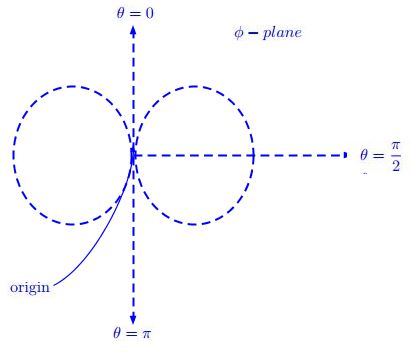
\includegraphics[width=.8\linewidth]{./graphics/diagram3a}
\caption{Radiation pattern of th E-plane.}
\label{figure14a}
\end{minipage}
\hfill
\begin{minipage}[b]{0.4\textwidth}
\includegraphics[width=.8\linewidth]{"./graphics/3D view radiation pattern"}
\caption{3D view of the radiation pattern.}
\label{figure14b}
\end{minipage}
\end{figure}

The 3D view of the radiation pattern is gotten by revolving figure \ref{figure14a} in the $\phi$ direction about it's axis since the electric field is symmetrical about the $\phi$ plane and it is shown in \ref{figure14b}

Notice that the antenna size is not shown in these figures because it is taken as a point and the field which is radiated from that point is plotted with its amplitude as a function of $\theta \ and \ \phi$ and the shape of the plot would look like an apple, figure \ref{figure15}. This is the radiation pattern of the Hertz dipole. Drawing the 3 dimensional variation of the field is rather tedious, instead, the plot of the radiation pattern is taken across two sections of the 3D view on a principal $\theta$ plane and a principal $\phi$ plane where we essentially capture the information of the radiation pattern on these planes. If we consider any arbitrary point on the 3D figure, the plane passing through that point and through the axis (at the origin) is $\theta$ - plane while a horizontal plane parallel to the xy or perpendicular to the $\theta$ plane that passes through the point is the $\phi$ plane. 

In our analysis, the $\theta$ - plane has only the $\theta$ component of the fields and for the Hertz dipole it is the electric field and it was plotted in figure \ref{figure14a}. This plane can now be called the E - plane and its plot is the radiation pattern of the E - plane. Also the $\phi$ plane has only the $\phi$ components the fields and it is the magnetic field $\vec{H}$. A plot of the radiation pattern on this plane is a circle. Suppose we cut \ref{figure14b} at $\theta$ = $\dfrac{\pi}{2}$ horizontally. The plot is shown in figure \ref{figure15}.
% INCLUDE FIGURE 15 HERE
\begin{figure}[h]
\centering
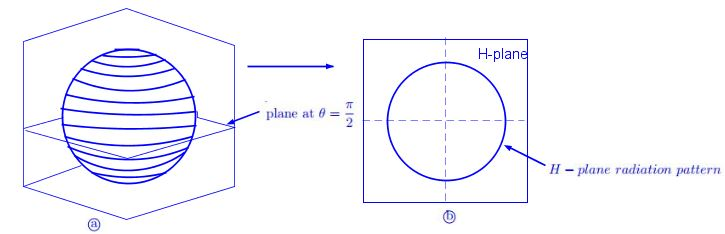
\includegraphics[width=0.8\linewidth]{./graphics/diagram4}
\caption{Radiation pattern of the H - plane}
\label{figure15}
\end{figure}

We call the plane the H - plane and the variation of the electric field on this plane is called the H - plane radiation pattern. 

So far, we have analyzed the field of the hertz dipole and have gotten the radiation pattern of the dipole in the 3D view as well as in the principal planes (E \& H). We observed that the H - plane radiation pattern is circular. This pattern is due to the symmetry of the Hertz dipole. In further analysis of circularly symmetric antennas like the linear dipole which we will treat later, we could always assume that the H - plane radiation pattern is always a circle. So, basically, we would be considering the E - plane radiation patterns but it is important to always visualize the 3D figure.

The radiation pattern is a very important aspect of an antenna because it shows the direction of power flow. For the Hertz dipole, it is seen that the maximum power flow is at $\theta = \dfrac{\pi}{2}$ (as $P \propto  |E|^2 $) and zero power flow is at $\theta\ =\ 0 \ or\ \theta\ =\ \pi $ as seen by the E - plane radiation pattern. It essentially shows that at the axis of the dipole there is no power flow and maximum power is radiated perpendicular to that axis. This shows that the dipole has a preferred direction for radiation of power. We remember that the Hertz dipole is the simplest possible antenna and it has a preferred direction for transfer of power. Hence, it will be very difficult to realize an antenna that transfers power uniformly in all directions (i.e it is isotropic). The directional dependence of an antenna is the direction of power flow. The application matters in the choice of an antenna, for an application where communication is established between two points, a highly directional antenna is used such as the microwave towers. Another instance, is the broadcasting station. A radio station needs to distribute information to a region in all directions, so it requires an isotropic antenna, but we have established that such an antenna is never possible. An antenna with characteristics that match such requirements is the Hertz dipole or linear dipole. Though it is not uniform in the E - plane, however, it is isotropic in the H - plane. 

The hertz dipole is not a practical antenna and so it is not useful. So we will consider a practical antenna of a length of wire and apply the condition for uniform current distribution ($\ell \ll \lambda$) where l is the length of the wire. Then, we will analyze it as a collection of small Hertz dipole and will be treated in the next chapter.